% !TeX root = ../../PRES.tex
    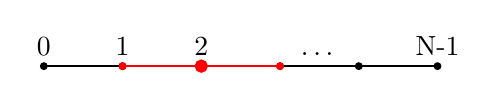
\begin{tikzpicture}[thick,>=latex,scale=1,l/.style={latex-latex},F/.style={-latex,very thick},v/.style={-latex',thick},
			vc/.style={-latex',thick,color=gray},d/.style={thin},w/.style={fill=white}] 
  \begin{scope}
	\draw(0,0)--+(5,0);
 	\foreach \i in {0, 1, ...,5} {
        	\visible<3->{\filldraw(\i,0) circle (1pt);}

      	  }
 	\foreach \i in {0, 1, ...,2} {
	\visible<4->{\draw(\i,0)node[above]{\i};}
}
	\visible<4->{\draw(5,0)node[above]{N-1};}
	\visible<4->{\draw(3.5,0)node[above]{\ldots};}
	\visible<5->{\draw[red](1,0)--+(1,0);
			\filldraw[red](2,0) circle (2pt);
			\draw[red](2,0)--+(1,0);
			}
        	\visible<6->{\filldraw[red](1,0) circle (1pt);}
        	\visible<6->{\filldraw[red](3,0) circle (1pt);}
    \end{scope}
    \end{tikzpicture}